\chapter{Software application} \label{chap:td:software}
\begin{figure}[ht]
	\centering
	\begin{tikzpicture}[
		% define box styles
		boxr/.style={rectangle, thick, draw=red!50!black, fill=red!5, minimum size=5mm},
		boxg/.style={rectangle, thick, draw=green!50!black, fill=green!5, minimum size=5mm},
		boxb/.style={rectangle, thick, draw=blue!50!black, fill=blue!5, minimum size=5mm},
		]
		% draw MW nodes
		\node[boxg] (ad2)								{Analog Discovery 2};
		\node[boxg] (app)		[above=of ad2] 			{Application};
		% draw main system nodes
		\node[boxb] (driver) 	[below=of ad2]			{Current driver};
		\node[boxb] (laser) 	[right=40 pt of driver]	{Laser};
		\node[boxb] (nv) 		[right=of laser] 		{NV sample};
		\node[boxb] (detect) 	[right=of nv]			{\textbf{Photodetector}};
		\node[boxg] (lockin)	[above=of detect]		{Lock-in amplifier};
		
		
		% draw app lines
		\draw[->, thick]			(app.south) 		to node[midway, left]{\glsfmtshort{ttl}}	(ad2.north);
		\draw[->, thick]			(ad2.north) 		to node[midway, right]{Oscilloscope}		(app.south);
		% draw main system lines
		\draw[->, thick]			(ad2.south)			to node[midway, left]{\glsfmtshort{ttl}} 	(driver.north);
		\draw[->, thick] 			(driver.east) 		to node[midway, above]{Current} 			(laser.west);
		\draw[->, thick]			(laser.east) 		to node[midway, above]{Light} 				(nv.west);
		\draw[->, thick]			(nv.east) 			to node[midway, above]{Light}				(detect.west);		
		\draw[->, thick]			(detect.north) 		to node[midway, right]{Signal}				(lockin.south);	
		% draw long lines
		\draw[->, thick] (ad2.east) to node[midway, below]{Reference signal} (lockin.west);
		\draw[->, thick] (lockin.west) to node[midway, above]{Processed photodetector data}(ad2.east);
	\end{tikzpicture}
	\caption{Overview of the $T_1$ measurements quantum sensing setup}
	\label{fig:td:ad2}
\end{figure}

A quick look at the goals laid out in Chapter \ref{chap:goals} makes it clear that they separate the pulsing sequence software from the \gls{daq} software. Despite this, during talks with the client it was decided that a \gls{gui} application that performs both functions also needed to be added to the task list. The main reason for this is that an all-encompassing application will make it easier for physics students with little coding experience to interact with the setup. This is also the reason why the application was implemented as a \gls{gui} instead of a \gls{cli}, which is easier to program, but can be harder to use. Another reason for integrating pulse generation and data acquisition is that, instead of reading data directly from the \gls{lia}, its output can be connected to the oscilloscope of the Analog Discovery. Because the application only needs to interact with one device, a single \gls{api} needs to be used and consequently coding separate applications will only result in a lot of copied code and a less user-friendly experience. 

While a single application for both functionalities is possible, different quantum protocols require different physical setups. This makes it is difficult to foresee what hardware changes are implemented and as a result only one protocol can be implemented at a time. With this information in mind, the client requested a Python application based on the Tk \gls{gui} kit that combines $T_1$ measurements pulse generation and data acquisition using the \gls{ad2}. 

A high-level diagram of the setup the application is written for can be seen in Figure \ref{fig:td:ad2}. This is the same setup originally shown in Figure \ref{fig:fd:t1_block} when the $T_1$ protocol was introduced. The only difference is the waveform generator and \gls{daq} blocks are replaced by the applications and the \gls{ad2} controlled by it.

% Thorlabs Photodiodes and Photoconductors Tutorial:
% https://www.thorlabs.com/newgrouppage9.cfm?objectgroup_id=9020
\section{Driving the laser} \label{chap:fd:laser_driver}
As discussed in Chapter \ref{specifications}, the laser driver has already been designed and built to drive the laser with a 5 \unit[]{\volt}. It gets \gls{ttl} signals from a waveform generator (the \gls{ad2} in this case) and outputs current to drive the connected laser.

Тhe designer explicitly states that tests were only done with frequencies of up to 100 \unit{\kilo\hertz} \cite{sitnic2023}. This is insufficient for the project, as for example, the pulsing sequence for $T_1$ measurements use pulses with duration of 5 \unit{\micro\second} (200 \unit{\kilo\hertz}) and downtime of as little as 1 \unit{\micro\second} (1 \unit{\mega\hertz})\footnote{These values are taken from Sewani et al \cite{sewani2020coherent}, but the clients intends to make the timings used by the quantum sensing setup even faster at some point in the future}. However, after a discussion with the original designer it was clarified that the driver should perform well enough for the needs of the setup. Furthermore, an improved version was made by a Smart Solutions Semester group. The redesigned board can drive the laser at 500 \unit{\kilo\hertz} with little to no distortion.

Previously, $T_1$ measurements and Rabi oscillations were mentioned when discussing pulsed protocols. Chapter \ref{chap:fd:t1} presented an overview of the $T_1$ pulsing scheme, which were implemented for the laser driver. Unfortunately, due to the high-frequency signal distortion of the Analog Discovery signals, only sequences for $T_1$ measurements were made, as other protocols have higher frequency requirements and require more analog output ports than the \gls{ad2} has.

The \gls{lia} reference signal can easily be generated by the \gls{ad2} using the Waveforms software. This is not the case for the laser driver signal. Waveforms supports custom sequence programming, however the system for writing these sequences only allows for pulses, which have a minimum duration $\tau_{las min}$ for which $\tau_{las min} \geq \frac{T_{seq}}{100}$ holds true\footnote{$T_{seq}$ is the period of the whole sequence}. It should also be noted that using the built-in pulse generation functionalities only allow for pulse durations that fit the formula $\tau_{las} = t_{las}\frac{T_{seq}}{100}$, where $t_{las} \in \mathbb{Z}^+$ and $t_{las} \leq 100$. These restrictions make it impossible for pulsing sequences to be designed in Waveforms. Thankfully, the \gls{ad2} software can read \gls{csv} files, which makes it possible to customize a sequence more freely.


\begin{figure}[ht]
	\centering
	\begin{tikzpicture}[
		% define box styles
		boxa/.style={rectangle, thick, draw=purple!50!black, fill=gray!5, minimum size=20mm},
		boxb/.style={rectangle, thick, draw=gray!50!white, fill=gray!5, minimum size=20mm},
		]
		% draw source/scope nodes
		\node[boxa] (b1)								{1};
		\node[boxb] (b2)		[right=0 mm of b1] 		{0};
		\node[boxb] (b3) 		[right=0 mm of b2]		{0};
		\node[boxa] (b4) 		[right=0 mm of b3]		{1};
		\node[boxb] (b5) 		[right=0 mm of b4]		{0};
	\end{tikzpicture}
	\caption{Example of a filled sequence buffer}
	\label{fig:td:driver:working_principle}
\end{figure}

But before delving into implementation details, the working of pulse generation in Waveforms needs to be discussed. An example of a filled Waveforms buffer, is shown Figure \ref{fig:td:driver:working_principle}. A \gls{ttl} signal can be generated using the values from it by setting the period $T_{seq}$ of the sequence and the peak voltage $V_{max}$. Those two values are necessary, because the buffer contains normalized values. In the example, each element has a value of either 0 or 1, which translate to 0 or $V_{max}$ when entered into the function generator. Furthermore, each pulse has a duration of $\tau_{las} = \frac{T_{seq}}{5}$.

A MATLAB script (see Figure \ref{code:t1_pulse} for full script) was written to generate buffer values based on the pulse duration $\tau_{las}$, the scaling factor $\gamma = \frac{T_{seq}}{\tau_{las}}$ and the normalized dark time $t_d = \frac{\tau_{d}}{\tau_{las}}$. Figure \ref{fig:fd:waveformssequence} shows a $T_1$ sequence where $\tau_{las}$ = 20 \unit{\micro\second}, $T_{seq}$ = 30 \unit{\milli\second} and $\tau_{d}$ = 200 \unit{\micro\second} (consequently $\gamma$ = 1500 and $t_d$ = 10). 

\begin{figure}[ht]
	\centering
	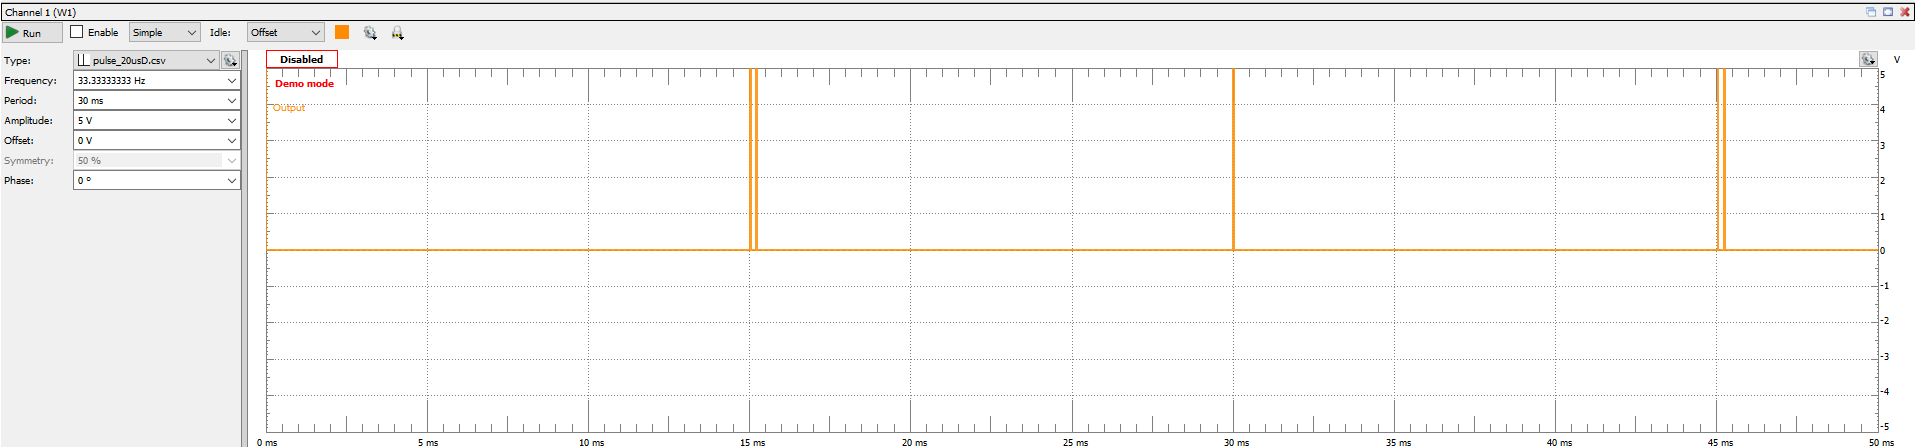
\includegraphics[width=1\linewidth]{img/waveforms_sequence}
	\caption{Waveforms function generator view after importing a $T_1$ pulse sequence}
	\label{fig:fd:waveformssequence}
\end{figure}


\section{\glsfmtshort{gui}}
Figure \ref{fig:td:appgui} shows what the front-end looks like when running the application. There are four panels that make up the program window: the device panel, the status log, the parameter panel and lastly the result plot.

\begin{figure}[ht]
	\centering
	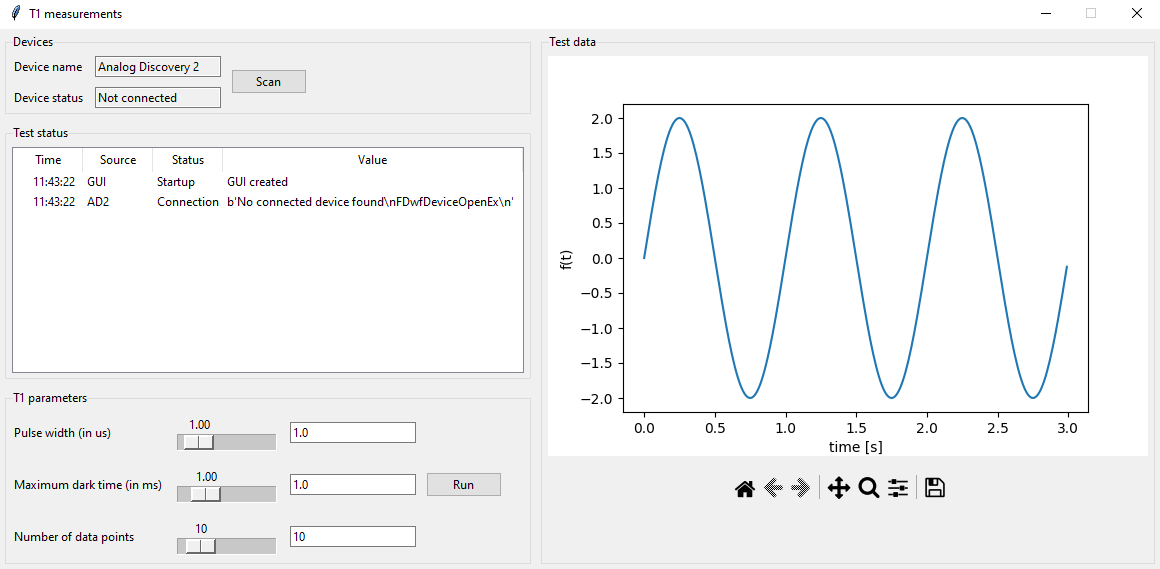
\includegraphics[width=1\linewidth]{img/app_gui}
	\caption{The \gls{gui} of the $T_1$ measurements application}
	\label{fig:td:appgui}
\end{figure}

The device panel is there to monitor the connection with the \gls{ad2}. On startup, a scan is conducted to find a device, but devices can also be plugged in later and, after pressing scan, the test can be ran. If no device is connected, the tests cannot be ran.

As Figure \ref{fig:td:appgui} shows, the status log contains messages pertaining to different subsystems. In addition to system statuses, it also tracks tests by reporting which data point is being executed at a given time. If there are any issues with the Analog Discovery while running $T_1$ measurements, they will be shown in the log as well.

Perhaps most important is the $T_1$ parameter panel. It allows the user to set custom values for tests. The minimum laser pulse width $\tau_{las}$ is set manually, but it also implicitly sets the sequence period $T_{seq}$ and the minimum dark time $\tau_{dmin}$ according to Equation \eqref{eq:td:tlas}. Setting the maximum dark time $\tau_{dmax}$ can also be done from this panel, however it should be noted that it cannot exceed $2000\tau_{dmin}$. The number of data points, or alternatively the number of dark times for which the test needs to be ran, can also be set. Based on the provided number, an array of dark times will be generated and then used when creating the sequences.

\begin{equation}\label{eq:td:tlas}
	\tau_{las} = 5\tau_{dmin} = \frac{T_{seq}}{819,2}
\end{equation}

The last panel contains the final $T_1$ plot. After running all data points and measuring the results, a plot of the dark times $\tau_d$ and their respective signal magnitude will be plotted. As of finalizing the report, the physical setup is incomplete, so the plot is only an example of how a \lstinline|numpy| plot will be rendered by the application.


%\section{Device connection}
%There are two events that call the function that connects to an Analog Discovery: startup and pressing the "Scan" button (see Figure \ref{fig:td:appgui}). It is important to verify the Analog Discovery connection before running $T_1$ measurements by scanning for devices, because there is no disconnection handler and even if the device was connected on startup, there is no guarantee it will be connected before running the test.
%
%\begin{figure}[ht]
%	\begin{lstlisting}[language=pythe]
%def find_device(self):
%	# version required for operation
%	version = create_string_buffer(16)
%	dwf.FDwfGetVersion(version)
%		
%	# define behavior on close (0 = run, 1 = idle, 2 = off)
%	dwf.FDwfParamSet(DwfParamOnClose, c_int(0))
%		
%	# open device and get interface reference
%	dwf.FDwfDeviceOpen(c_int(-1), byref(self.hdwf))
%		
%	# disable auto config for better performance
%	dwf.FDwfDeviceAutoConfigureSet(self.hdwf, c_int(0))
%	\end{lstlisting}
%	\caption{Simplified device discovery and connection function}
%	\label{fig:td:find_device}
%\end{figure}
%
%A simplified version of the connection method that does not handle connection errors can be seen in Figure \ref{fig:td:find_device}. What the snippet of code shows is the required \gls{api} calls. After retrieving the library version, the device is configured so that, even if the program is exited, the inputs and outputs will finish executing and measuring the current $T_1$ sequence. Afterwards, the first device that is found is opened and its handle is passed to the instance of the application class. Finally, the last line of code disables automatic reconfiguration. It is important that it is turned off, otherwise the device will be reconfigured on every call to a \lstinline|FDwf*Set| function, which will significantly worsen the performance of the Analog Discovery.


%\section{Message logging}
%The message log is an important medium for communicating with the user. As previously mentioned, the log contains status messages from the different subsystems of the application, in addition to the $T_1$ measurement information.  Logging is done to a \lstinline|ttk.Treeview|\footnote{The code in Figure \ref{fig:td:treeview} uses a \lstinline|ttk| widget, which is not one of the standard \lstinline|tk| widgets. \lstinline|ttk|, aside from providing extra widgets, offers more modern versions of many \lstinline|tk| widgets, which is why it is used whenever possible.} widget, which is configured to function like a table. Figure \ref{fig:td:treeview} shows how the tree is created and assigned to the \lstinline|tree_running_log| attribute. After the \gls{gui} is created, a message is logged using the \lstinline|log_message| method to notify the user.
%
%\begin{figure}[ht]
%	\begin{lstlisting}[language=pythe]
%# create tree
%self.tree_running_log = ttk.Treeview(lf_status, columns=("Source", "Status", "Value"))
%		
%# log first status message
%self.log_message("GUI", "Startup", "GUI created")
%	\end{lstlisting}
%	\caption{Simplified message log widget creation}
%	\label{fig:td:treeview}
%\end{figure}
%
%Figure \ref{fig:td:log_message_function} contains the code for logging a message. A call to the function should contain the source, status (also known as short message) and value (also known as long message). There are several log sources. \lstinline|GUI| indicates a message is about \lstinline|tkinter| or more broadly about the \gls{gui} application. If the source is \lstinline|AD2|, then the message is about the device status. Furthermore, if the Analog Discovery sends an error (e.g. data loss) during execution, it will be logged as \lstinline|AD2|. Messages about the status of the $T_1$ measurements are logged with the sources set to \lstinline|T1|.
%
%\begin{figure}[ht]
%	\begin{lstlisting}[language=pythe]
%def log_message(self, source, status, value):
%	timestamp = datetime.now().strftime("%H:%M:%S")
%	self.tree_running_log.insert('', tk.END, text=timestamp, values=(source, status, value))
%	\end{lstlisting}
%	\caption{Simplified message logging function}
%	\label{fig:td:log_message_function}
%\end{figure}


\section{Pulse generation}
The fundamentals of pulse generation using the Analog Discovery, which were laid out in Chapter \ref{chap:fd:laser_driver}, still hold true, even when using the WaveForms \gls{sdk} for Python.

That being said, there is one major difference. The buffer size, which was limited to 100 when set through the WaveForms app, is actually 4096. This allows for pulse durations that fit the formula $\tau_{las} = t_{las}\frac{T_{seq}}{4096}$, for $t_{las} \in \mathbb{Z}^+$ and $t_{las} \leq 4096$.

As a consequence of the similarities, the MATLAB code for pulse generation from Chapter \ref{chap:fd:laser_driver} (see Figure \ref{code:t1_pulse}) was rewritten in Python, with the calls to the WaveForms \gls{api} replacing the \gls{csv} file writer. 

Before doing anything else, the pulse generation function calls the function for determining the dark time for every data point. Ideally, this function would return many small values and some bigger ones. Such data point spacing can be achieved using \lstinline|numpy.logspace|, which provides logarithmically-spaced values, thus satisfying the aforementioned conditions. Despite its theoretical applicability, in actuality it cannot be used because it is designed with floating-point numbers in mind. In this case, the buffer slot count $t_d$ is a rounding of the actual dark time $\tau_d$, which makes them integers. Additionally, rounding functions cannot be used in combination with \lstinline|numpy.logspace|, because for a lot of data points, the function can return multiple of the same $t_d$, which is not desirable. To get around these problems, a function based on \lstinline|numpy.logspace| was implemented. 

\begin{equation}\label{eq:logpspace_custom}
	t_{d} = t_{dmin} + round(10^{x\frac{\log(t_{dmax})}{n - 1}})\ for\ x \in [1,n]\cap \mathbb{Z}
\end{equation}

\begin{figure}[ht]
	\begin{lstlisting}[language=pythe]
def gen_log_space(self, td_min, td_max, n):
	result = [td_min]
	# return 1 if bad n
	if n <= 1:
		return result
		
	for i in range(1, n):
		td_curr = td_min + round(10 ** (i * log10(td_max) / (n - 1)))
		# exits prematurely if min and max are too close, otherwise replaces last value with td_max
		if td_curr >= td_max:
			result.append(td_max)
			return result
		
		# check if dark time is repeating last value and increment if yes
		if td_curr - result[-1] >= 1:
			result.append(td_curr)
		else:
			result.append(result[-1] + 1)
	return result
	\end{lstlisting}
	\caption{Custom \lstinline|logspace| function implementation}
	\label{fig:td:logspace_gen_func}
\end{figure}


Equation \eqref{eq:logpspace_custom} shows that, provided with the minimum and maximum dark time $t_{dmin}$ and $t_{dmax}$, as well as the number of data points $n$, the function returns logarithmically-spaced values. To address the problem with repetitions, $t_d$ is incremented whenever it is equal to the $t_d$ of the previous data point. This increment, however, results in the final value being bigger than the $t_{dmax}$. In the worst case, this might result in writing data outside the buffer range, which is why the last value is manually set to $t_{dmax}$. 


Figure \ref{fig:td:logspace_gen_func} shows the custom \lstinline|logspace| function. To compare its performance to the original function, the plots in Figure \ref{fig:td:logspace} were made. It is clear that both functions demonstrate similar behaviors for big values, but the custom function also presents linear behavior for low $t_d$ values, as can be seen in Figure \ref{fig:td:logspace_small}.


\begin{figure}[!ht]
	\centering
	\begin{subfigure}[1a]{.49\linewidth}
		\centering
		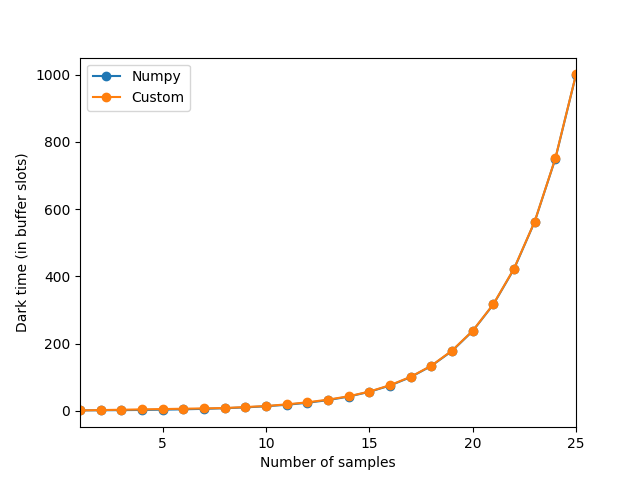
\includegraphics[width=\linewidth]{matlab/logspace_large_td}
		\caption{Plot of all 25 data points}
		\label{fig:td:logspace_whole}
	\end{subfigure}
	\hfill
	\begin{subfigure}[1b]{.49\linewidth}
		\centering
		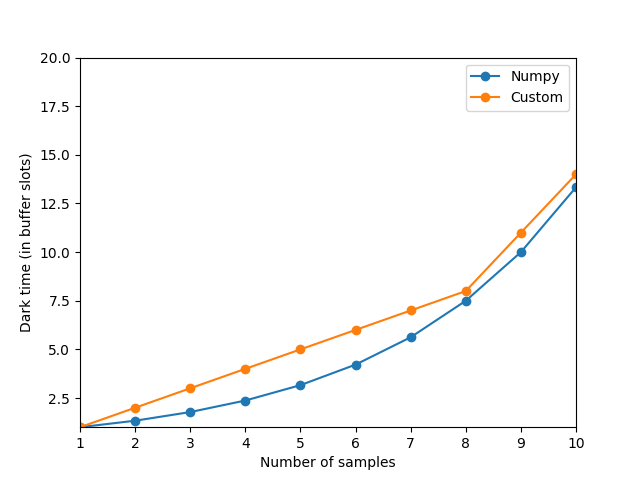
\includegraphics[width=\linewidth]{matlab/logspace_small_td}
		\caption{Plot of the first 10 data points}
		\label{fig:td:logspace_small}
	\end{subfigure}
	\caption{Generating buffer dark times $t_{d}$ using \lstinline|numpy.logspace| and a custom function from 1 to 1000 with 25 data points}
	\label{fig:td:logspace}
\end{figure}


After calculating the buffer space required for all dark times, the sequences can be generated. As previously mentioned, setting the pulse duration $\tau_{las}$ implicitly determines the minimum dark time $\tau_{dmin}$ and the period of the sequence $T_{seq}$ based on the ratio $\tau_{las}:\tau_{dmin}:T_{seq} = 5:1:4096$. With only these ratios, and the already computed dark times, the sequence can be generated as shown in the snippet of code in Figure \ref{fig:td:sequence_gen_loop}. In it, \lstinline|pw| is the pulse width (5 buffer slots), \lstinline|pattern_size| is the buffer size attribute (fixed to 4096 slots) and \lstinline|all_tds| is the array of dark times (smallest value is 1 buffer slot).


\begin{figure}[ht]
	\begin{lstlisting}[language=pythe]		
# make pattern
for curr_td in all_tds:
	pattern = (c_double * self.pattern_size)(0)  # initialize C-style zero array
	# make pulse duration equal to pw
	for i in range(0, pw):
		# cancellation pulse
		pattern[i] = 1  
		# initialization pulse
		pattern[i + int(self.pattern_size / 2)] = 1  
		# readout pulse
		pattern[i + pw + curr_td + int(self.pattern_size / 2)] = 1 
	# save sequence to attribute 
	self.sequences.append(pattern)
	\end{lstlisting}
	\caption{Loop which generates an array of C-style arrays filled with binary buffer values}
	\label{fig:td:sequence_gen_loop}
\end{figure}

%Following the sequence generation, the Analog Discovery has to be configured for outputting the sequences. The code in Figure \ref{fig:td:pulsing_sequence} shows the \gls{api} calls that are needed when \lstinline|hdwf| attribute is a handle to the same device that was opened during device discovery and the \lstinline|laser_channel| is a waveform generator channel that is a attribute assigned to the class in its constructor. \lstinline|dwf.FDwfDeviceAutoConfigureSet| is disabled. First the \lstinline|laser_channel|, which is the attribute assigned to the laser pulsing waveform generator channel, is enabled. After that, the function of the waveform generator needs to be set. \gls{ttl} pulses use the custom analog function, which is called \lstinline|funcCustom| and it allows for writing patterns to the buffer. What follows is a call to the function for setting the buffer data using a $T_1$ sequence loaded in \lstinline|pattern|, which has the fixed length of 4096. Afterwards, the frequency of the whole pattern needs to be set to the pattern frequency \lstinline|f_pattern|, which is calculated based on the minimum pulse time. Here it should be noted that the buffer contains normalized values, which means that the following setting of the amplitude is required. The \lstinline|amplitude| variable passed to the \gls{api} call is 5 \unit{\volt} and should not be changed, unless the laser and laser driver change. Then the waveform generator can start outputting the current $T_1$ sequence until, at the end of the sequence, the output is reset. This whole process is done for every data point. Lastly, it is important to mention that all the functions which are called with \lstinline|AnalogOutNodeCarrier| as a parameter need it, as it tells them to configure the signal and not the channel modulation.


%\begin{figure}[ht]
%	\begin{lstlisting}[language=pythe]		
%dwf.FDwfAnalogOutNodeEnableSet(self.hdwf, self.laser_channel, AnalogOutNodeCarrier, c_int(1)) # enable
%dwf.FDwfAnalogOutNodeFunctionSet(self.hdwf, self.laser_channel, AnalogOutNodeCarrier, funcCustom) # set function to custom
%dwf.FDwfAnalogOutNodeDataSet(self.hdwf, self.laser_channel, AnalogOutNodeCarrier, pattern, c_int(self.pattern_size)) # set pattern of custom function
%dwf.FDwfAnalogOutNodeFrequencySet(self.hdwf, self.laser_channel, AnalogOutNodeCarrier, c_double(f_pattern)) # set frequency of the whole pattern
%dwf.FDwfAnalogOutNodeAmplitudeSet(self.hdwf, self.laser_channel, AnalogOutNodeCarrier, amplitude) # set amplitude of the whole pattern to 5V
%dwf.FDwfAnalogOutConfigure(self.hdwf, self.laser_channel, c_int(1)) # start outputting
%# execute some other code here
%dwf.FDwfAnalogOutReset(self.hdwf, self.laser_channel)
%	\end{lstlisting}
%	\caption{Outputting the first sequence from the \lstinline|sequences| attribute of the \gls{gui} object using the WaveForms \gls{api}}
%	\label{fig:td:pulsing_sequence}
%\end{figure}

%Configuring the lock-in reference channel to output a square-wave signal is quite similar, which is why the code for it was put in Appendix \ref{chap:appendix:code} (Figure \ref{code:sequence_gen_loop}). The only difference is the waveform generator function type, which is provided to \lstinline|dwf.FDwfAnalogOutNodeFunctionSet|. Instead of a custom analog function, the square wave \lstinline|funcSquare| type is passed. Afterwards there is no pattern to set, so there is no call to \lstinline|FDwfAnalogOutNodeDataSet|.

\section{Data acquisition} \label{chap:td:daq}
To measure test data in the simplest way possible, it is crucial that whatever \gls{lia}[] is used to extract the photodetector signal outputs to the Analog Discovery oscilloscope, as shown in Figure \ref{fig:td:ad2}. This allows for the use of the same Waveforms \gls{api} that handles waveform generation.

There are several acquisition modes supported by the \gls{ad2}, but only two were found to meet the needs of the sensing setup. \lstinline|acqmodeSingle| is the primary \gls{daq} mode. As the name suggests, it records a single buffer of a certain length when triggered. In contrast, \lstinline|acqmodeRecord| records data for a given number of seconds by constantly overwriting the same buffer. For the purposes of this project, streaming data with \lstinline|acqmodeRecord| is more practical, as it allows an experiment to be run for a variable number of seconds instead of having only a single \gls{daq} buffer to work with. A sampling rate of 5 \unit[]{\mega\hertz} was chosen to meet the needs of $T_1$ measurements. Though this sampling frequency is theoretically sufficient for supporting the $T_1$ protocol, it is not enough for measuring Rabi oscillations, which requires 10 \unit{\mega\hertz} at least. This is not an issue for the current \gls{daq} implementation, as $T_1$ measurements is its sole focus, but this means future projects will not be able to use the \gls{ad2} for data acquisition.

After concluding the reading of a data point, the whole stream of data is stored to a \gls{csv} file, which can then be used for processing and plotting. The \gls{csv} file format was chosen as an intermediary to make the code more modular by separating the data acquisition and processing. This way, a different \gls{daq} system with a different \gls{api} can replace the current one without needing to modify the data processing module.

%The oscilloscope channel setup, which is used for data acquisition, requires setup that is somewhat reminiscent of the waveform generator setup, as is evident from Figure \ref{fig:td:daq_setup}. As before, the oscilloscope first needs to be enabled. Afterwards, its signal range has to be set, which is the maximum value that it can read. Then the mode of operation of the oscilloscope needs to be configured. \lstinline|acqmodeRecord| tells the Analog Discovery that it needs to stream in data continuously. Alternatively, it is possible to use single acquisition with \lstinline|acqmodeSingle|, however this imposes a limit on the amount of data, as well as its resolution. Following the acquisition mode configuration, the mode-specific settings need to be configured. Firstly, the sampling frequency of the oscilloscope needs to be set. This value cannot exceed the clock. Additionally, if there is missing or corrupted data in the streamed buffer, then the sampling rate needs to be lowered, because it is the only possible culprit. Secondly, the recording length has to be configured by setting it in seconds. After the mode-specific configuration, a call to \lstinline|FDwfAnalogInConfigure| needs to be made in order to reset the trigger. By setting the reconfigure flag to \lstinline|c_int(1)| and the start flag to \lstinline|c_int(0)|, the data acquisition is not started and the device trigger is reset. It is mandatory to wait for a period of time afterwards and the Waveform \gls{sdk} documents usually set that period of time to 2 seconds. To start the data acquisition, a similar call to \lstinline|FDwfAnalogInConfigure| needs to be made, except the values of the reconfigure and start flags are swapped. Just like before, \lstinline|hdwf| is the device handle received on opening the Analog Discovery and \lstinline|scope_channel| is a channel enumeration constant.

%\begin{figure}[ht]
%	\begin{lstlisting}[language=pythe]		
%dwf.FDwfAnalogInChannelEnableSet(self.hdwf, self.scope_channel, c_int(1)) # enable oscilloscope (acquisition) channel
%dwf.FDwfAnalogInChannelRangeSet(self.hdwf, self.scope_channel, amplitude) # set the vertical range of the oscilloscope to 5V
%dwf.FDwfAnalogInAcquisitionModeSet(self.hdwf, acqmodeRecord) # set the mode of the oscilloscope to record (continuously streaming data)
%dwf.FDwfAnalogInFrequencySet(self.hdwf, c_double(daq_sf)) # set the sample frequency of the acquisition to 5MHz
%dwf.FDwfAnalogInRecordLengthSet(self.hdwf, c_double(run_time)) # set the length of the recording to equal that of the run time (or -1 for infinite recording length)
%dwf.FDwfAnalogInConfigure(self.hdwf, c_int(1), c_int(0)) # reset trigger timeout
%time.sleep(wait_time) # wait for offset to stabilize
%dwf.FDwfAnalogInConfigure(self.hdwf, c_int(0), c_int(1)) # enable
%	\end{lstlisting}
%	\caption{Configuring an oscilloscope channel using the WaveForms \gls{api}}
%	\label{fig:td:daq_setup}
%\end{figure}
%
%While the loop used to retrieve data from the stream is somewhat complicated, it is essentially made up of the code in Figure \ref{fig:td:daq_read}. The status of data stream needs to be retrieved first. This is done by calling \lstinline|FDwfAnalogInStatusRecord|, which writes the number of available, lost and corrupted samples to the pointers provided to it. After getting the recording status, \lstinline|FDwfAnalogInStatusData| is called to copy all the available samples into the stream output buffer \lstinline|daq_buffer|. After concluding the reading, the whole stream of data is stored to a \gls{csv} file, which can then be used for processing and plotting.
%
%\begin{figure}[ht]
%	\begin{lstlisting}[language=pythe]		
%dwf.FDwfAnalogInStatusRecord(self.hdwf, byref(s_available), byref(s_lost), byref(s_corrupted)) # retrieve information about data loss and corruption
%# code for handling lost/corrupted data goes here
%dwf.FDwfAnalogInStatusData(self.hdwf, self.scope_channel, byref(daq_buffer, sizeof(c_double) * daq_samples_read), s_available) # get scope channel data and copy it to the buffer
%	\end{lstlisting}
%	\caption{Reading from oscilloscope using the WaveForms \gls{api}}
%	\label{fig:td:daq_read}
%\end{figure}


\section{Data processing and visualization}
\begin{figure}[!ht]
	\centering
	\begin{subfigure}[1a]{.49\linewidth}
		\centering
		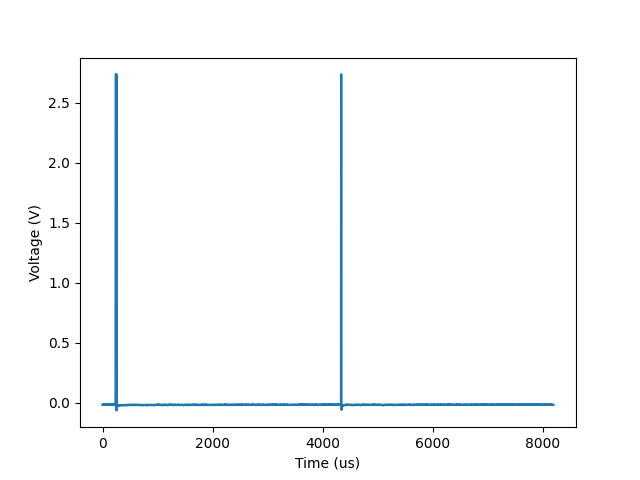
\includegraphics[width=\linewidth]{matlab/t1_pulse}
		\caption{Plot of all pulses in one period}
		\label{fig:td:t1_visualization_whole}
	\end{subfigure}
	\hfill
	\begin{subfigure}[1b]{.49\linewidth}
		\centering
		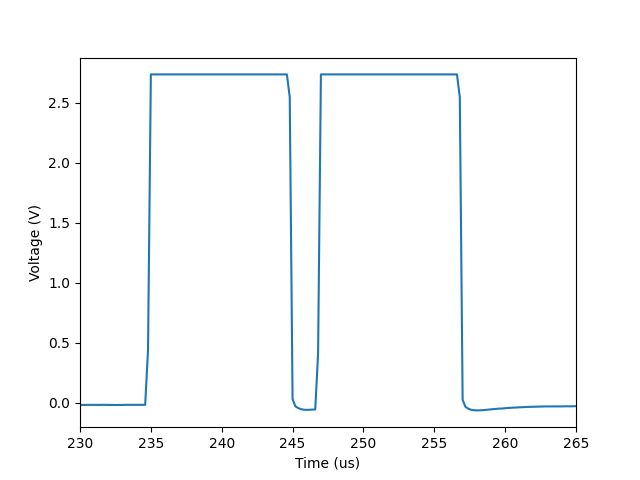
\includegraphics[width=\linewidth]{matlab/t1_pulse_zoom}
		\caption{Plot of the initialization and readout pulses}
		\label{fig:td:t1_visualization_zoom}
	\end{subfigure}
	\caption{Plots of the pulsing sequence of the first data point when running the test with 10 \unit{\micro\second} pulse width $\tau_{las}$ and 2 \unit{\micro\second} minimum dark time $\tau_{dmin}$ with a sampling rate of 5 \unit{\mega\hertz}}
	\label{fig:td:t1_visualization}
\end{figure}

As of finalizing the report, the $T_1$ measurements setup has still not been assembled and, consequently, limited data processing could be done. That being said, data processing and visualization has still been considered and the groundwork has been laid out by using mock data.

To simulate the signal that would be read during a $T_1$ measurement, the oscilloscope can be connected directly to the waveform generator while it is outputting $T_1$ pulsing sequences. Figure \ref{fig:td:t1_visualization} shows plots of a pulsing sequence data point. In Chapter \ref{chap:td:daq}, it was shown that the data acquisition is set to a time period in seconds. In that amount of time, many $T_1$ measurements will need to be done. Literature on $T_1$ relaxometry needs to be consulted for a formula to convert the light intensity changes to a single number per measurement, as Formula \eqref{eq:t1}, which was provided in Chapter \ref{chap:fd:t1}, is only theoretical and implementing it in practice is not trivial. Afterwards, the average of all measurements needs to be taken. Combining the averages of all data points in one plot should result in a plot like Figure \ref{fig:t1result}. 
